\chapter{Interaction discovery for logistic regression} \label{chap5}

\epigraph{.}{.}

\minitoc


\textcolor{red}{needs quote}

\textit{Nota Bene :} Ce chapitre s'inspire fortement ... \textcolor{red}{à adapter au moment de l'envoi du manuscrit}

\bigskip

\selectlanguage{english}

Continuing my pursuit of interpretable representation learning algorithms for \gls{lr}, I tackle in this chapter a common problem in \textit{Credit Scoring} and other application contexts relying either on \gls{lr} or additive models of the form $f(y) = \sum_{j=1}^d \glssymbol{bth}_j' \q_j(x_j)$. To further reduce the model bias discussed in Section~\ref{chap1:sec3} and thus obtain better predictive performance while maintaining interpretability, \textit{Credit Scoring} practitioners are used to introducing pairwise interactions.


\section{Motivation: XOR function}

As described in the introduction, \gls{lr} is linear in its inputs which does not allow to take into account conditional dependency: the change of slope of a feature's log-odds given another (moderator) feature (see~\cite{berry2010testing}). This problem is often dealt with by sparsely introducing ``interactions'', \textit{i.e.}\ products of two features. Unfortunately, this leads again to a model selection challenge as the number of pairs of features is $\dfrac{d(d-1)}{2}$. Let $\bdelta$ denote the triangular inferior matrix with $\delta_{k,\ell} = 1$ if $k < \ell$ and features $k$ and $\ell$ ``interact'' in the \gls{lr} in the sense of~\cite{berry2010testing}. The \gls{lr} with interactions $\bdelta$ is thus:
\begin{equation} \label{eq:reglog_sans}
\text{logit}[p_{\glssymbol{bth}}(1|\q(\glssymbol{bx}),\bdelta)] = \theta_{0} + \sum_{j=1}^d \glssymbol{bth}_j' \q_j(x_j) + \sum_{1 \leq k < \ell \leq d} \delta_{k,\ell} \sigma( \glssymbol{bth}_{k,\ell} \odot \q_k(x_k) \q_\ell(x_\ell)' ),
\end{equation}
where $\odot$ denotes the element-wise (Hadamard) matrix multiplication (already used in Chapter~\ref{chap1}), $\sigma(\cdot)$ the sum of all elements of a matrix (used here only for notational convenience since all matrices of coefficients of pairwise interactions have varying dimensions), $\glssymbol{bth}_{k,\ell} = (\theta_{k,\ell}^{r,s})_{1 \leq r \leq m_k, 1 \leq s \leq m_\ell}$ and for all features $j$, $m_j$ is set as the ``reference'' value and consequently for all $j$, $\theta_{j}^{m_j}=0$ and for all $1 \leq k < \ell \leq d$, $\theta_{k,\ell}^{m_k,m_{\ell}}=0$. Since, in presence of an interaction between $k$ and $\ell$, $\theta_{k}$ already encodes the log-odd ratio of feature $k$ conditionally to $\ell$ being at its reference value $m_\ell$, $\theta_{k,\ell}^{1,m_\ell},\dots,\theta_{k,\ell}^{m_k-1,m_\ell}$ are redundant and thus set to $0$. Note that the ``main effect'' $\theta_k$ could have been removed altogether instead (which is the classical, in-house formulation of interactions at \gls{cacf}) but since interactions will be added / removed  back and forth, the present formulation seems more adequate.

This formulation seems rather complicated visually and in terms of parameter dimension: a single interaction between two quantized features (or more broadly speaking, categorical features) amounts to adding $(m_k - 1) \cdot (m_\ell - 1)$ coefficients. Since ``interpretable'' were advocated, \textit{i.e.}\ sparse, simple models to yield scorecards as in Table~\ref{tab:ex_scorecard}, and a high variance was displayed, when estimating numerous coefficients, on Figure~\ref{fig:sinus_fin}, it does not seem like a good idea. As a side note, interpretation of the resulting parameters can be rather tricky. The monographs~\cite{jaccard2003interaction,james2001interaction} were really helpful and are sincerely recommended to the interested reader.

Nevertheless, as thoroughly explained in~\cite{berry2010testing}, there are situations where interactions terms are unavoidable. A simple (but quite extreme) example is the XOR (exclusive or) function $f(x_1,x_2) = (x_1 + x_2)\cdot(2 - x_1 - x_2)$ where $x_1,x_2 \in \{0,1\}$. Such functions cannot be learnt by a standard \gls{lr}. For a more illustrative example, the broad field of medicine is often interested in knowing the factors of risks of a given disease and if these factors have additive or cumulative effects (see~\cite{morgan2014adversity} for an example), \textit{e.g.}\ risk of contracting disease A is doubled with factors B and C individually, but 6 times more when both factors are present. This is precisely what is observed in the \textit{Credit Scoring} industry: higher risk is observed among workers than executives but when associated with the time spent in the current job position, workers with ``stability'' of employment may appear less risky than less ``stable'' executives in a non-additive way.

Moreover, the number of coefficients is nevertheless kept low by having few levels, as emphasized in Chapter~\ref{chap4}, and few interactions, as emphasized by the $\bdelta$ notation. Additionally and traditionally in \textit{Credit Scoring}, so-called ``main-effects'', \textit{i.e.}\ features $\q_k(x_k)$ and $\q_\ell(x_\ell)$ are removed when their interaction term is present ($\delta_{k,\ell} = 1$). In biostatistics, it is usually the contrary (interactions are only considered when main effects are present), as will be seen in the following Section, where a literature review is given, alongside a reformulation of the problem.


\section{Pairwise interaction screening as a feature selection problem}

Criterion~\eqref{eq:BICq} developed in the context of quantization can be adapted to take into account interactions:
\begin{equation} \label{eq:criterion_inter}
\q^\star,\bdelta^\star = \argmin_{\q,\bdelta} \text{BIC}(\hat{\glssymbol{bth}}_{\q,\bdelta}),
\end{equation}
where $\hat{\glssymbol{bth}}_{\q,\bdelta}$ is the MLE of $\glssymbol{bth}$ given $(\glssymbol{bbx},\glssymbol{bby})$, $\q$ and $\bdelta$. Supplemental to the \nameref{par:consistency} of Section~\ref{par:consistency}, $\delta_{k,\ell}$ is an estimated parameter of the model and an additional $\frac{d(d-1)}{2}$ term shall be added to the penalization term $\nu_\q$ of the BIC criterion~\eqref{eq:BICq}. The combinatorics involved in this problem are much higher than those of criterion~\eqref{eq:BICq}, which already lead to an untractable greedy approach. For each feasible quantization scheme of Section~\ref{par:cardinality}'s ~\nameref{par:cardinality}, there is now $2^{\frac{d(d-1)}{2}}$ models to test! In this section, the discretization will first be considered fixed and a stochastic approach similar to the one proposed for discretization and grouping of factor levels is developed.

With a fixed discretization scheme $\q$, criterion~\ref{eq:criterion_inter} amounts to $\bdelta^\star = \argmin_{\bdelta} \text{BIC}(\hat{\glssymbol{bth}}_{\q,\bdelta})$ which optimization through a greedy approach is untractable with more than a few features ($d > 10$). The first approach that seems straightforward in this setting is to simply see all $\frac{d(d-1)}{2}$ interactions as features to select from. In this potentially high-dimensional parameter space, the most computationnaly-effective approach is to resort to penalization. Various penalization approaches have been developed recently, among which LASSO~\cite{tibshirani1996regression} and its derivatives can effectively perform feature selection. A CIFRE PhD has even been dedicated to the subject with application to \textit{Credit Scoring}~\cite{vital2016} as was explained in Chapter~\ref{chap1}.

The penalization approach has been applied to the interaction screening problem, very often in biostatistics-related problems, \textit{e.g.}\ gene-gene interactions. Its first use~\cite{park2007penalized} relies on $L^2$ regularization, for stability of estimation of the large number of coefficients, and forward stagewise selection of features to avoid a phenomenon where an interaction between a meaningful feature and a meaningless one would remain in the model: it would imply that the main effect coefficient of the meaningful feature could be lower, and thus preferable w.r.t.\ the $L^2$ penalty. The LASSO has been applied to this problem as well~\cite{wu2009genome} by first selecting features with the LASSO based solely on main effects, then selecting pairwise interactions among the selected main effects, again with the LASSO, which requires all main effects of the considered interactions to be present in the model. Rather than conducting such a two-stage procedure, which might greatly influence the considered interactions and does not work under the ``weak hierarchy'' hypothesis (only one of the features of a pairwise interaction need to be present as a main effect), a set of convex constraints is added to the LASSO in~\cite{bien2013lasso} such that main effects and pairwise interactions are selected in a one-shot procedure with the hierarchy constraint. In a different setting, with much stricter hypotheses on the data, namely that they are Gaussian for each class, a statistical test involving the sample pairwise correlations is derived in~\cite{simon} to characterize the probability of an interaction.

Model-free approaches have been proposed in the biostatistics literature (\cite{yang2008snpharvester,zhang2010team,li2013model,dong2008exploration,zhang2007bayesian,wan2010boost} and references therein) where focus is given to large $d$, small $n$ settings. Moreover, these approaches are not multivariate (\textit{i.e.}\ other features than the ones involved in the pair that is tested are discarded) and are not directly applicable to a particular predictive model $p_{\glssymbol{bth}}$. Since interaction screening will be considered alongside quantization, these methods are thus discarded from the present study.


\section{A novel model selection approach}

I take another approach here, which foremost benefit will appear in the subsequent Section, and which closely resembles the strategy employed in the quantization setting of Chapter~\ref{chap4} and in particular Section~\ref{sec:sem}. The variable $\bdelta$ can be seen as an observation of a latent random matrix so that a stochastic approach can be used to search for $\bdelta^\star$.

\subsection{Relation of the BIC criterion and the interaction probability}

The BIC criterion has a desirable property, from a Bayesian perspective, relating it to the likelihood of the data given the model (in our case, a given interaction matrix $\bdelta$) given the data (see~\cite{lebarbier}), where the parameter space $\Theta$ depends on the model $\bdelta$:
%\begin{align*}
%p(\glssymbol{bbx},\glssymbol{bby} | \bdelta) & = \int_{\Theta} p(\glssymbol{bbx},\glssymbol{bby} | \glssymbol{bth}) p(\glssymbol{bth} | \bdelta)d\glssymbol{bth} \\
%& = \exp(-\text{BIC}(\hat{\glssymbol{bth}}_{\bdelta})/2 + O(1))
%\end{align*}
\begin{align*}
p(\glssymbol{bbx}, \glssymbol{bby} | \bdelta) & = \int_{\Theta} p_{\glssymbol{bth}}(\glssymbol{bbx}, \glssymbol{bby} | \bdelta) p(\glssymbol{bth} | \bdelta)d\glssymbol{bth} \\
 & = \int_{\Theta} p_{\glssymbol{bth}}(\glssymbol{bby} | \glssymbol{bbx}, \bdelta) p(\glssymbol{bth} | \bdelta) p(\glssymbol{bx}) d\glssymbol{bth} \\
\ln p(\glssymbol{bbx}, \glssymbol{bby} | \bdelta) & = \int_{\Theta} \ln p_{\glssymbol{bth}}(\glssymbol{bby} | \glssymbol{bbx}, \bdelta) p(\glssymbol{bth} | \bdelta) d\glssymbol{bth} + \ln p(\glssymbol{bx}) \\
 & = -\text{BIC}(\hat{\glssymbol{bth}}_{\bdelta})/2 + \ln p(\glssymbol{bx}) + O(1)
\end{align*}
Replacing the features $\glssymbol{bbx}$ by their (fixed) quantized version $\q(\glssymbol{bbx})$ and rewriting the posterior probability of the model by introducing the preceding likelihood, we get:
\begin{align*}
p(\bdelta | \q(\glssymbol{bbx}),\glssymbol{bby}) & \propto p(\glssymbol{bby} | \q(\glssymbol{bbx}), \bdelta) p(\bdelta) \\
& \approx \exp(-\text{BIC}(\hat{\glssymbol{bth}}_{\q,\bdelta})/2) p(\bdelta)
\end{align*}

\subsection{Metropolis-Hastings sampling algorithm}

This Section is dedicated to describing the Metropolis-Hastings~\cite{hastings1970monte} sampling algorithm that will be used in the next section to sample from $p(\bdelta | \q(\glssymbol{bbx}),\glssymbol{bby})$ that will be denoted, for simplicity, by $\pi(\bdelta)$ in this Section.

The distribution $\pi(\bdelta)$ is not known explicitly but $f(\bdelta) = \exp(-\text{BIC}(\hat{\glssymbol{bth}}_{\q,\bdelta})/2) p(\bdelta)$ is proportional to $\pi(\bdelta)$. Consequently, given two matrices $\bdelta,\bdelta'$, the \gls{pdf} ratio is the same: $\frac{\pi(\bdelta)}{\pi(\bdelta')} = \frac{f(\bdelta)}{f(\bdelta')}$.

Now suppose we have at our disposal a proposal distribution of the form:
\begin{alignat}{2}
\tr: \; & ({\{0,1\}}^{\frac{d(d-1)}{2}},{\{0,1\}}^{\frac{d(d-1)}{2}}) && \mapsto \mathbb{R} \nonumber \\ 
& (\bdelta,\bdelta') && \to \tr(\bdelta,\bdelta') = \tr(\bdelta' | \bdelta) \nonumber
\end{alignat}
This instrumental conditional distribution will be used to design an MCMC which empirical distribution of drawn matrices $\bdelta^{(0)}, \dots, \bdelta^{(\text{iter})}$ approaches $\pi(\bdelta)$. The \gls{sem} algorithm in Section~\ref{sec:sem} followed the same strategy. The algorithm is the following:

\begin{algorithm}[H]
 \KwData{$f, \tr, \text{max\_iter}$}
 \KwResult{$ \bdelta^{(0)}, \dots, \bdelta^{(\max\_\text{iter})} $}
 Initialization of $ \bdelta^{(0)} \sim p(\bdelta)$\;
 $s = 0$\;
 \While{$s < \text{max\_iter} $}{

Draw $\bdelta' \sim \tr(\cdot | \bdelta^{(s)})$\;

Calculate the acceptance probability $\alpha = \max \left( 0, \min \left( 1, \frac{f(\bdelta')}{f(\bdelta^{(s)})} \frac{\tr(\bdelta' | \bdelta^{(s)})}{\tr(\bdelta^{(s)} | \bdelta')} \right) \right) $\;

%\uIf{$\alpha \geq 1$}{
%Let $\bdelta^{(s+1)} \leftarrow \bdelta'$\;
%}
%\Else{
%Let $\bdelta^{(s+1)} \leftarrow \begin{cases} \bdelta' \text{ with probability } \alpha, \\ \bdelta^{(s)} \text{ with probability } 1-\alpha.  \end{cases}$\;
%}
Let $\bdelta^{(s+1)} \leftarrow \begin{cases} \bdelta' \text{ with probability } \alpha, \\ \bdelta^{(s)} \text{ with probability } 1-\alpha.  \end{cases}$\;
}
\caption{\label{metropolis} Metropolis-Hastings (the $\max$ and $\min$ functions enforce $0 \leq \alpha \leq 1$).}
\label{alg:metro}
\end{algorithm}

This algorithm reaches asymptotically the target distribution $\pi(\bdelta)$ if such a stationary distribution exists and is unique~\cite{meyn2012markov}. ``Detailed balance'' is a sufficient but not necessary condition of existence according to which each transition $\bdelta^{(s)} \rightarrow \bdelta^{(s+1)}$ is reversible. Uniqueness is guaranteed if the resulting Markov Chain is ergodic. This is satisfied if every interaction matrix $\bdelta$ is aperiodic and positive recurrent (\text{i.e.}\ each matrix $\bdelta \in {\{0,1\}}^{\frac{d(d-1)}{2}}$ is reachable in a finite number of iterations). 

It is also important to notice that, apart from verifying the above assumptions, there are no guidelines about how to choose the proposal distribution or the number of iterations necessary for proper estimation. These are ``hyperparameters'' that may influence greatly the effectiveness of the method.

\subsection{Designing an MCMC sampling of good interactions} \label{subsec:mcmc}

It follows from the preceding Section that one can design an MCMC algorithm like Metropolis-Hastings~\eqref{alg:metro} which draws ``good'' interaction matrices $\bdelta$ from the target posterior distribution $p(\bdelta | \glssymbol{bbx},\glssymbol{bby})$.

\subsubsection{Transition probability}

Metropolis-Hastings only requires a proposal of a transition probability between two matrices of the Markov chain that was denoted by $\tr$. This approach would require to compute $2^{d(d-1)}$ probabilities (\textit{i.e.}\ one per unique couple of matrices ($\bdelta,\bdelta'$)). It is thus desirable to reduce this combinatorics by making further assumptions. In what follows, possible transitions are restricted to matrices that are on a one unit $L^{1,1}$ distance (sum of all absolute entries) to the current interaction matrix, or equivalently which belong to the $\left( \frac{d(d-1)}{2}-1 \right)$-sphere of center $\bdelta$ denoted by $S^{\left( \frac{d(d-1)}{2}-1 \right)}_{\bdelta}$: 
\begin{align*}
\tr(\bdelta,\bdelta') = 0 & \text{ if } \sum_{k=1}^d \sum_{\ell=1}^d |\delta_{k,\ell} - \delta'_{k,\ell}| \neq 1 \\
 & \equiv ||\bdelta - \bdelta'||_{1,1} \neq 1 \\
 & \equiv \bdelta' \not\in S^{\left( \frac{d(d-1)}{2}-1 \right)}_{\bdelta}.
\end{align*}
Only $\frac{d(d-1)}{2}$ coefficients are now needed, which can be reinterpreted as the probability to switch on (resp. off) an entry of $\bdelta$ which is currently off (resp. on). It can be claimed that a good intuition about whether two features interact is the relative gain (or loss) in BIC between their bivariate model \textit{with} their interaction and this model \textit{without} their interaction. The rationale behind such a procedure, relying again on the properties of BIC, is the following: 
%\begin{align*}
%\forall \: 1 \leq k < \ell \leq d, \; p(\delta_{k,\ell} | \q_k(\glssymbol{bbx}_k), \q_\ell(\glssymbol{bbx}_\ell), \glssymbol{bby}) & \propto p(\q_k(\glssymbol{bbx}_k), \q_\ell(\glssymbol{bbx}_\ell), \glssymbol{bby} | \delta_{k,\ell}) p(\delta_{k,\ell}) \\
%& \approx \exp(-\text{BIC}(\hat{\glssymbol{bth}}_{\q_k,\q_\ell,\delta_{k,\ell}})/2) p(\delta_{k,\ell}).
%\end{align*}
\begin{align*}
\forall \: 1 \leq k < \ell \leq d, \; p(\delta_{k,\ell} | \q_k(\glssymbol{bbx}_k), \q_\ell(\glssymbol{bbx}_\ell), \glssymbol{bby}) & \propto p(\glssymbol{bby} | \q_k(\glssymbol{bbx}_k), \q_\ell(\glssymbol{bbx}_\ell), \delta_{k,\ell}) p(\delta_{k,\ell}) \\
& \approx \exp(-\text{BIC}(\hat{\glssymbol{bth}}_{\q_k,\q_\ell,\delta_{k,\ell}})/2) p(\delta_{k,\ell}).
\end{align*}

Setting a uniform prior $p(\delta_{k,\ell}=1) =\begin{cases} 0 \text{ if } k \geq \ell \\ \frac{1}{2} \text{ otherwise} \end{cases}$ and denoting by $p_{k,\ell}$ the probability of an interaction given features $\q_k(x_k)$ and $\q_\ell(x_\ell)$:
\begin{equation} \label{eq:pkl}
p_{k,\ell} = p(\delta_{k,\ell} = 1 | \q_k(\glssymbol{bbx}_k), \q_\ell(\glssymbol{bbx}_\ell), \glssymbol{bby}) \appropto \exp \left( \frac{\text{BIC}(\hat{\glssymbol{bth}}_{\q_k,\q_\ell,\delta_{k,\ell}=0}) - \text{BIC}(\hat{\glssymbol{bth}}_{\q_k,\q_\ell,\delta_{k,\ell}=1})}{2} \right)
\end{equation}
The $p_{k,\ell}$ are normalized s.t.\ $\sum_{1 \leq k < \ell \leq d} p_{k,\ell} = 1$ and denote their triangular inferior matrix arrangement by $P$. Note that in this setting, $p_{k,\ell}$ involves nested models that were discussed in Section~\nameref{par:consistency} such that the consistency of the BIC criterion is assured whatever multiplicative constant to the number of parameters $\nu_\q$ is used. It can be claimed that if $p_{k,\ell}$ is close to $1$ (resp. $0$), then there is a strong chance that $\delta_{k,\ell}^\star = 1$ (resp. $\delta_{k,\ell}^\star = 0$) even in the full multivariate model, which amounts to:
\[ p_{k,\ell} \approx p(\delta_{k,\ell} = 1 | \q(\glssymbol{bbx}),\glssymbol{bby}) \]
This holds in particular if features $\q_k(\glssymbol{bbx}_k)$ and $\q_\ell(\glssymbol{bbx}_\ell)$ are independent to other features $\q_{-\{k,\ell\}}(\glssymbol{bbx}_{-\{k,\ell\}})$:
\begin{align*}
p(\delta_{k,\ell} | \q(\glssymbol{bx}),y) & = \frac{p(y , \q(\glssymbol{bx}), \delta_{k,\ell})}{p(y , \q(\glssymbol{bx}))} \\
 & = \frac{p(y | \q(\glssymbol{bx}),\delta_{k,\ell}) p(\delta_{k,\ell}, \q(\glssymbol{bx}))}{p(y,\q(\glssymbol{bx}))} \\
 & = \frac{p(\q_{k,\ell}(\glssymbol{bx}_{k,\ell}),\delta_{k,\ell} | y) p(\q_{-\{k,\ell\}}(\glssymbol{bx}_{-\{k,\ell\}}) | y) p(y) p(\delta_{k,\ell},\q_{k,\ell}(\glssymbol{bx}_{k,\ell})) p(\q_{-\{k,\ell\}}(\glssymbol{bx}_{-\{k,\ell\}})) }{p(y,\q(\glssymbol{bx})) p(\q_{k,\ell}(\glssymbol{bx}_{k,\ell}),\delta_{k,\ell}) p(\q_{-\{k,\ell\}}(\glssymbol{bx}_{-\{k,\ell\}}))} \\
 & = \frac{p(y | \q_{k,\ell}(\glssymbol{bx}_{k,\ell}),\delta_{k,\ell}) p(\q_{-\{k,\ell\}}(\glssymbol{bx}_{-\{k,\ell\}}) | y) p(\delta_{k,\ell},\q_{k,\ell}(\glssymbol{bx}_{k,\ell}))}{p(\q_{-\{k,\ell\}}(\glssymbol{bx}_{-\{k,\ell\}}) | y) p(\q_{k,\ell}(\glssymbol{bx}_{k,\ell}) | y) p(y) } \\
 & = \frac{p(y | \q_{k,\ell}(\glssymbol{bx}_{k,\ell}),\delta_{k,\ell}) p(\delta_{k,\ell},\q_{k,\ell}(\glssymbol{bx}_{k,\ell}))}{p(y , \q_{k,\ell}(\glssymbol{bx}_{k,\ell}))} \\
 & = p(\delta_{k,\ell} | \q_{k,\ell}(\glssymbol{bx}_{k,\ell}), y)
\end{align*}
Note also that in this setting and for $n \to +\infty$, the first step of the Metropolis-Hastings described hereafter suffices since the $p_{k,\ell}$ converge to $\delta_{k,\ell}^\star$ thanks to the properties of the BIC criterion.

Consequently, if at step $(s)$ of the Markov chain, $\delta_{k,\ell}^{(s)} = 1$ (resp. $0$) and $p_{k,\ell}$ is close to $0$ (resp. $1$), a good candidate for $\bdelta^{(s+1)}$ should be to change $\delta_{k,\ell}$ to $\delta_{k,\ell}^{(s+1)} = 0$ (resp. $\delta_{k,\ell}^{(s+1)} = 1$). Our proposal is thus to calculate the difference between the current interaction matrix and $P$ which is denoted by $\tr^{(s)} = |\bdelta^{(s)} - P|$ and normalize.

This defines a proper transition probability between two interaction matrices:
\[ \tr(\bdelta^{(s)},\bdelta') = \begin{cases} 0 \text{ if } ||\bdelta^{(s)} - \bdelta'||_{1,1} \neq 1, \\ \tr^{(s)} \odot |\bdelta^{(s)} - \bdelta'|. \end{cases} \]

\subsubsection{Acceptance probability of the proposed transition}


Following Algorithm~\eqref{alg:metro}, a Metropolis-Hastings step can now be conducted by drawing $\bdelta' \sim \tr(\bdelta^{(s)},\cdot)$. The acceptance probability of this candidate is given by:
\begin{align*}
\alpha & = \max \left( 0, \min \left( 1, \frac{p(\bdelta' | \q(\glssymbol{bbx}), \glssymbol{bby})}{p(\bdelta^{(s)} | \q(\glssymbol{bbx}), \glssymbol{bby})} \frac{1-\tr(\bdelta^{(s)},\bdelta')}{\tr(\bdelta^{(s)},\bdelta')} \right) \right) \\
& \approx \max \left( 0, \min \left( 1, \exp \left( \frac{\text{BIC}(\hat{\glssymbol{bth}}_{\q(\glssymbol{bbx}),\delta_{k,\ell}=0}) - \text{BIC}(\hat{\glssymbol{bth}}_{\q(\glssymbol{bbx}),\delta_{k,\ell}=1})}{2} \right) \frac{1-\tr(\bdelta^{(s)},\bdelta')}{\tr(\bdelta^{(s)},\bdelta')} \right) \right).
\end{align*}
It must here be remarked that by construction of $\tr^{(s)}$ and the transition probability $\tr(\bdelta^{(s)},\bdelta')$, we have $\tr(\bdelta',\bdelta^{(s)}) = 1 - \tr(\bdelta^{(s)},\bdelta')$. Still following Algorithm~\eqref{alg:metro}, the candidate $\bdelta'$ is accepted with probability $\alpha$ s.t.\ $\bdelta^{(s+1)} = \begin{cases} \bdelta' \text{ with probability } \alpha, \\ \bdelta^{(s)} \text{ with probability } 1-\alpha. \end{cases}$

\subsubsection{Validity of the approach}


The existence of the stationary distribution $p(\bdelta | \q(\glssymbol{bbx}),\glssymbol{bby})$ is guaranteed by construction of the Metropolis-Hastings algorithm as the generated Markov chain fulfills the detailed balance condition. The uniqueness of the stationary distribution is given by the ergodicity of the Markov chain: as $\forall \: 1 \leq  k < \ell \leq d, \: \tr_{k,\ell}^{(s)} > 0$ and a transition changes only one entry $\delta_{k,\ell}$ of the interaction matrix, every state can be reached in at most $\frac{d(d-1)}{2}$ steps.

In practice with a fixed discretization scheme, this stochastic approach is probably outperformed in computing time by LASSO-based methods or correlation-based methods like~\cite{simon}, which might obtain a suboptimal model in a fixed computing time, contrary to our approach which might take lots of steps to converge in distribution. Its double benefit however lies in the ability of the practitioner to define before-hand how many steps shall be performed and the natural integration to the quantization algorithm proposed in the previous Chapter, which is developed in the next Section.

\section{Interaction screening and quantization}

We return to our original objective~\ref{eq:criterion_inter} and consider optimizing the BIC criterion both in terms of quantization and pairwise interactions, as varying the quantization $\q$ might influence the ``best'' interactions $\bdelta^\star$ and vice versa.

The MCMC approach proposed in the previous Section can be mixed with the \textit{glmdisc} algorithm proposed in the previous Chapter. A brute force way of doing this is to conduct a full MCMC search, as proposed in the previous Section, for each proposed quantization $\hat{\q}^{(t)}$ from Chapter~\ref{chap4} (either with the SEM or NN approach). Of course, this is too computationally intensive: our proposed Metropolis-Hastings algorithm necessitates the calculation of 2 univariate \gls{lr} per $p_{k,\ell}$ \textit{i.e.}\ $d(d-1)$ \gls{lr} and one multivariate \gls{lr} per step $s$. These $O(d^2 + \max\_{\text{iter}})$ \gls{lr} shall be estimated for each proposed quantization which itself requires the estimation of $O(d)$ softmax (see Section~\ref{subsec:relaxation}) or polytomous \gls{lr} and contingency table (see Section~\ref{subsec:fuzzy}).

The foremost bottleneck lies in the aforementioned initialization of the Metropolis-Hastings algorithm. In essence, the proposed initialization is not required: the closer the proposal distribution to the target distribution, the quicker the convergence, which was our aim with the formulation of $p_{k,\ell}$ in Equation~\eqref{eq:pkl}. However, the asymptotic convergence in distribution is nevertheless maintained whatever proposal distribution is used, provided the resulting Markov Chain has a unique stationary distribution. I will consequently design a proposal distribution of $\bdelta$ for all quantizations $\bqk \in \Q$. To still put ``\textit{prior}'' information (to the MCMC, it is not \textit{a priori} in the Bayesian sense) about potential interactions into it, the ``raw'' features can be used instead:
\begin{equation} \label{eq:pklnew}
p_{k,\ell} = p(\delta_{k,\ell} = 1 | \glssymbol{bbx}_k, \glssymbol{bbx}_\ell, \glssymbol{bby}) \appropto \exp \left( \frac{\text{BIC}(\hat{\glssymbol{bth}}_{x_k,x_\ell,\delta_{k,\ell}=0}) - \text{BIC}(\hat{\glssymbol{bth}}_{x_k,x_\ell,\delta_{k,\ell}=1})}{2} \right).
\end{equation}
The second bottleneck is the number of Metropolis-Hastings steps per \gls{sem} step. It must be remembered that these two MCMC algorithms are meant to be used for their asymptotic properties. The target distribution of $\q$ in the \gls{sem} algorithm is thought to be extremely dominated by $\q^\star$ as argumented in Section~\ref{subsec:fuzzy}, such that after some step $(s)$, proposed quantizations are very close to $\q^\star$ (and consequently very similar to each others) at which point the interaction screening algorithm while performing the quantization steps is somewhat similar to its ``static'' counterpart developed in the preceding Section.

As a consequence, a single interaction matrix can be proposed at each step of the \gls{sem}-Gibbs algorithm introduced in Section~\ref{sec:sem}. Apart from the initialization defined above, nothing changes in the \textit{glmdisc}-SEM algorithm: the \gls{sem}-Gibbs sampler allowed us to ``hold'' $\bqk_{-\{j\}}^{(s)}$ while drawing $\bqk_{j}^{(s+1)}$ for all features, resulting in $\bbqk^{(s+1)}$. Here, the same applies with $\bdelta$ that is drawn holding $\bbqk^{(s+1)}$. The formal algorithm is detailed in Appendix~\ref{app1:glmdiscSEM} and is reproduced partially hereafter.

First, $P$ is computed according to the formulation of $p_{k,\ell}$ given above in Equation~\eqref{eq:pklnew}.

Second, related to the Metropolis-Hastings algorithm, an initialization of the interaction matrix $\bdelta^{(0)}$ is done following a uniform distribution, as hypothesized earlier. Related to the \gls{sem} algorithm, $\bbqk^{(0)}$ is also initialized randomly.

Then, the \gls{sem} algorithm begins: following Section~\ref{sec:sem}, $\hat{\glssymbol{bth}}^{(s)}$ and $\hat{\ag}_j^{(s)}$ are respectively the MLE of $p_{\glssymbol{bth}}(y | \bqk^{(s)}, \bdelta^{(s)})$ (note the presence of $\bdelta$ here) and $p_{\ag_j}(\bqk_j | x_j)$ (strictly equivalent to the procedure without interactions).

The \gls{sem}-Gibbs sampler is still applicable: $\bqk_j$ is drawn knowing $\bqk_{-\{j\}}$ from $p_{\hat{\glssymbol{bth}}^{(s)}}(y | \bqk_{-\{j\}}^{(s)}, \cdot, \bdelta^{(s)}) p_{\hat{\ag}^{(s)}}(\cdot | x_j)$. At this point, $\bdelta^{(s+1)}$ can be computed from the Metropolis-Hastings algorithm similarly to the preceding Section. This procedure is iterated for a user-defined number of steps.

This procedure is much less costly than what could originally be thought of: the $d(d-1)$ \gls{lr} necessary to initialize the Metropolis-Hastings algorithm are still needed, but only once, and at each step, only one \gls{lr}, supplementary to the complexity of the original \textit{glmdisc}-SEM approach, is needed.

Focus is given to numerical experiments in the next Section on simulated, benchmark and real data.

%\begin{figure}
%\centering
%\resizebox{\linewidth}{6cm}{%
%% Created by tikzDevice version 0.11 on 2018-07-20 11:37:01
% !TEX encoding = UTF-8 Unicode
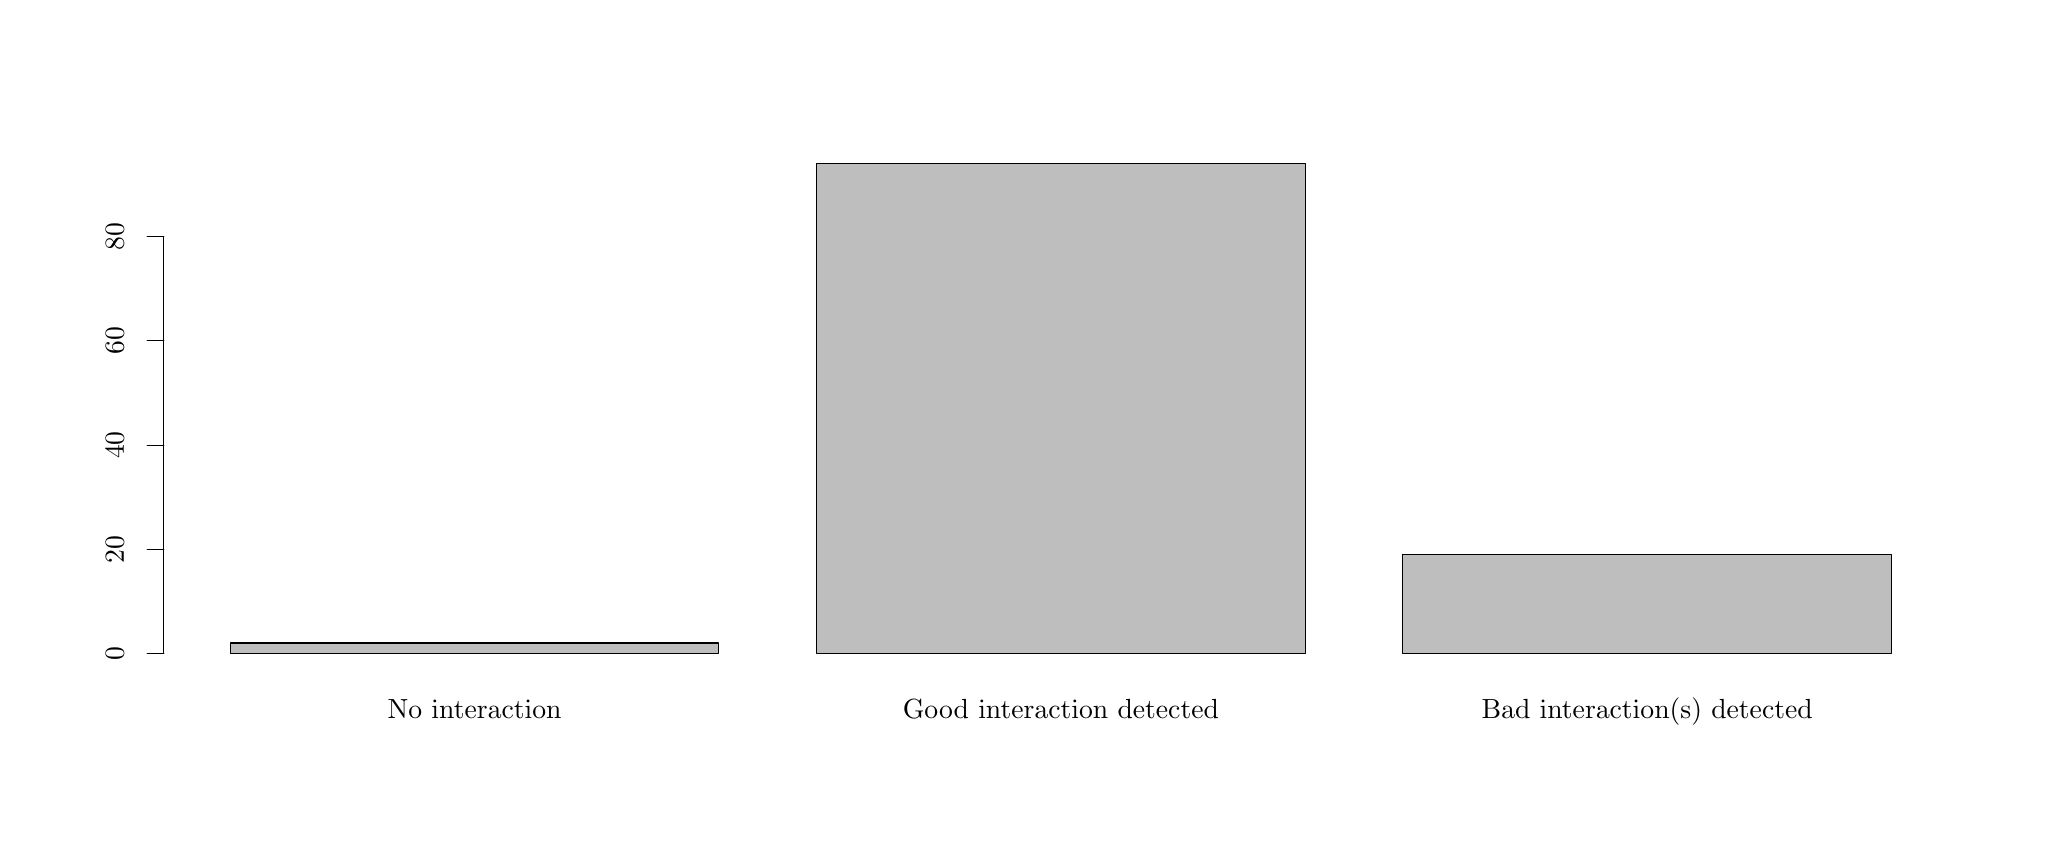
\begin{tikzpicture}[x=1pt,y=1pt]
\definecolor{fillColor}{RGB}{255,255,255}
\path[use as bounding box,fill=fillColor,fill opacity=0.00] (0,0) rectangle (722.70,289.08);
\begin{scope}
\path[clip] (  0.00,  0.00) rectangle (722.70,289.08);
\definecolor{drawColor}{RGB}{0,0,0}
\definecolor{fillColor}{RGB}{190,190,190}

\path[draw=drawColor,line width= 0.4pt,line join=round,line cap=round,fill=fillColor] ( 73.21, 62.97) rectangle (249.76, 66.73);

\path[draw=drawColor,line width= 0.4pt,line join=round,line cap=round,fill=fillColor] (285.07, 62.97) rectangle (461.63,239.88);

\path[draw=drawColor,line width= 0.4pt,line join=round,line cap=round,fill=fillColor] (496.94, 62.97) rectangle (673.49, 98.73);
\end{scope}
\begin{scope}
\path[clip] (  0.00,  0.00) rectangle (722.70,289.08);
\definecolor{drawColor}{RGB}{0,0,0}

\node[text=drawColor,anchor=base,inner sep=0pt, outer sep=0pt, scale=  1.00] at (161.49, 39.60) {No interaction};

\node[text=drawColor,anchor=base,inner sep=0pt, outer sep=0pt, scale=  1.00] at (373.35, 39.60) {Good interaction detected};

\node[text=drawColor,anchor=base,inner sep=0pt, outer sep=0pt, scale=  1.00] at (585.21, 39.60) {Bad interaction(s) detected};

\path[draw=drawColor,line width= 0.4pt,line join=round,line cap=round] ( 49.20, 62.97) -- ( 49.20,213.53);

\path[draw=drawColor,line width= 0.4pt,line join=round,line cap=round] ( 49.20, 62.97) -- ( 43.20, 62.97);

\path[draw=drawColor,line width= 0.4pt,line join=round,line cap=round] ( 49.20,100.61) -- ( 43.20,100.61);

\path[draw=drawColor,line width= 0.4pt,line join=round,line cap=round] ( 49.20,138.25) -- ( 43.20,138.25);

\path[draw=drawColor,line width= 0.4pt,line join=round,line cap=round] ( 49.20,175.89) -- ( 43.20,175.89);

\path[draw=drawColor,line width= 0.4pt,line join=round,line cap=round] ( 49.20,213.53) -- ( 43.20,213.53);

\node[text=drawColor,rotate= 90.00,anchor=base,inner sep=0pt, outer sep=0pt, scale=  1.00] at ( 34.80, 62.97) {0};

\node[text=drawColor,rotate= 90.00,anchor=base,inner sep=0pt, outer sep=0pt, scale=  1.00] at ( 34.80,100.61) {20};

\node[text=drawColor,rotate= 90.00,anchor=base,inner sep=0pt, outer sep=0pt, scale=  1.00] at ( 34.80,138.25) {40};

\node[text=drawColor,rotate= 90.00,anchor=base,inner sep=0pt, outer sep=0pt, scale=  1.00] at ( 34.80,175.89) {60};

\node[text=drawColor,rotate= 90.00,anchor=base,inner sep=0pt, outer sep=0pt, scale=  1.00] at ( 34.80,213.53) {80};
\end{scope}
\end{tikzpicture}

%}
%\caption{\label{fig:simulated_interaction} Distribution of the kind of interactions chosen by \textit{glmdisc} on 100 simulations.}
%\end{figure}
%
%
%
%
%\begin{figure}
%\centering
%\begin{tikzpicture}
%\tikzset{vertex/.style = {shape=circle,draw,minimum size=1.5em}}
%\tikzset{edge/.style = {->,> = latex'}}
%% vertices
%\node[vertex] (x1) at  (0,1.5) {$\glssymbol{X}_1$};
%\node[vertex] (xj) at  (0,0) {$\glssymbol{X}_j$};
%\node[vertex] (xd) at  (0,-1.5) {$\glssymbol{X}_{d}$};
%
%\node[vertex] (delta) at  (2.5,3) {$\bdelta$};
%
%\node[vertex] (q1) at  (2.5,1.5) {$Q_1$};
%\node[vertex] (qj) at  (2.5,0) {$Q_j$};
%\node[vertex] (qd) at  (2.5,-1.5) {$Q_{d}$};
%
%\node[vertex] (y) at (5,0) {$\glssymbol{Y}$};
%
%%edges
%%\draw[edge] (x1) to (delta);
%%\draw[edge] (xj) to (delta);
%%\draw[edge] (xd) to (delta);
%
%\draw[edge] (delta) to (y);
%
%\draw[edge] (x1) to (q1);
%\draw[edge] (xj) to (qj);
%\draw[edge] (xd) to (qd);
%\draw[edge] (q1) to (y);
%\draw[edge] (qj) to (y);
%\draw[edge] (qd) to (y);
%
%\draw[dashed] (x1) to (xj);
%\draw[dashed] (xj) to (xd);
%
%\draw[dashed] (q1) to (qj);
%\draw[dashed] (qj) to (qd);
%\end{tikzpicture}
%\caption{\label{fig:dep2} Dépendance entre $\glssymbol{X}_j$,$\Q_j$, $\bdelta$ et $\glssymbol{Y}$} 
%\end{figure}




\section{Numerical experiments}

In the same flavor as Chapter~\ref{chap4}, the proposed algorithm for interaction screening is first tested on simulated data, to show empirically its consistency, then on benchmark datasets and on \textit{Credit Scoring} data from~\gls{cacf} as in the previous Chapter. The same scheme is applied for the \textit{glmdisc} algorithm augmented with the interaction screening approach as described in the previous Section.
%For the sake of simplicity while reporting the results and of avoiding long implementation time on both proposed approaches, namely \textit{glmdisc}-SEM and \textit{glmdisc}-NN, these experiments rely exclusively on \textit{glmdisc}-SEM.
The code used for numerical experiments is available as packages, see Appendix~\ref{app2}.

\subsection{Simulated data}

In this first part, focus is given on showing empirically the consistency of the approach. The same data generation process as in Chapter~\ref{chap4} is employed: two continuous features $x_1$ and $x_2$ are sampled from the uniform distribution on $[0,1]$ and discretized as exemplified on Figure~\ref{fig:exp_sim} by using
\[\q_1(\cdot)=\q_2(\cdot) = (\mathds{1}_{]-\infty,1/3]}(\cdot),\mathds{1}_{]1/3,2/3]}(\cdot),\mathds{1}_{]2/3,\infty[}(\cdot)).\]
Here, following (\ref{eq:Cjhcont}), we have $d=2$ and $m_1=m_2=3$ and the cutpoints are $c_{j,1}=1/3$ and $c_{j,2}=2/3$ for $j=1,2$. Setting $\glssymbol{bth}^{1}=(0,-2,2,0,-2,2,0)$, $\bdelta^{1} = 0$, $\glssymbol{bth}^{2} = (\glssymbol{bth}^{1},)$, $\bdelta^{2} = 1$ the target feature $y$ is then sampled from $p_{\glssymbol{bth}^{o}}(\cdot | \q(\glssymbol{bbx}), \bdelta^{o}), o = \{1,2\}$ via the logistic model (\ref{eq:reglogq}). Two cases are first studied:
\begin{enumerate}[(a)]
    \item First, it is assessed that in the presence of a true interaction, it is discovered by our procedure, so that we simulate $Y \sim p_{\glssymbol{bth}^{2}}$ and provide $\q(\glssymbol{bbx})$;
    \item Second, it is assessed that in the absence of a true interaction, no interaction is found by our procedure, so that we simulate $Y \sim p_{\glssymbol{bth}^{1}}$ and provide $\q(\glssymbol{bbx})$.
\end{enumerate}
As promised, two further cases are first studied:
\begin{enumerate}[(a)]
    \item First, it is assessed that in the presence of a true interaction, it is discovered by \textit{glmdisc} while quantizing the data, so that we simulate $Y \sim p_{\glssymbol{bth}^{2}}$ and provide $\glssymbol{bbx}$;
    \item Second, it is assessed that in the absence of a true interaction, no interaction is found by \textit{glmdisc} while quantizing the data, so that we simulate $Y \sim p_{\glssymbol{bth}^{1}}$ and provide $\glssymbol{bbx}$.
\end{enumerate}
Note that the interaction screening procedure is also applicable to continuous features, which is not tested here. These 4 experiments are run 100 times with $n = \{1{,}000,10{,}000\}$ and histograms are given in Table~\ref{tab:simu_inter}.

\begin{table}[ht]
    \centering
    \caption{For \textit{glmdisc} w. and w.o. providing true quantization and different sample sizes $n$, (a) Bar plot of $\hat{\bdelta} = 0,1$ (resp.) for $\bdelta=1$. (C) Bar plot of $\hat{\bdelta} = 0,1$ (resp.) for $\bdelta=0$.}
    \label{tab:simu_inter}
\begin{tabular}{lllllll}
Algorithm & $n$ & (a) & $\hat{\bdelta}$ & (b) & $\hat{\bdelta}$ \\
\hline
\textit{glmdisc} w. provided quantization & $1{,}000$ & \myobar{9}{90}{1} & \mybar{60}{32}{8} \\
\textit{glmdisc} w.o. provided quantization & $1{,}000$ & \myobar{9}{90}{1} & \mybar{60}{32}{8} \\
\textit{glmdisc} w. provided quantization & $10{,}000$ & \myobar{0}{100}{0} & \mybar{88}{12}{0} \\
\textit{glmdisc} w.o. provided quantization & $10{,}000$ & \myobar{0}{100}{0} & \mybar{88}{12}{0}
\end{tabular}
\end{table}





\subsection{Benchmark datasets}

Table~\ref{tab:banchmark} (see Section~\ref{subsec:exp_benchmark} for details about the datasets) is complemented with the \textit{glmdisc}-SEM approach with interactions in the last column of Table~\ref{tab:banchmark_inter}.

\textcolor{red}{commenter les résultats exclusivement des interactions}

\begin{table}
    \centering
        \caption{Gini indices (the greater the value, the better the performance) of our proposed quantization algorithm \textit{glmdisc} and two baselines: ALLR and MDLP / $\chi^2$ tests obtained on several benchmark datasets from the UCI library.}
    \label{tab:banchmark_inter}
\begin{small}
\begin{tabular}{llllll}
Dataset & ALLR & \textit{ad hoc} methods & \makecell{Our proposal:\\ \textit{glmdisc}-NN} & \makecell{Our proposal:\\ \textit{glmdisc}-SEM} & \makecell{\textit{glmdisc}-SEM\\ w.\ interactions} \\
\hline
Adult & 81.4 (1.0) & \textbf{85.3} (0.9) & 80.4 (1.0) & 0 & \\
Australian & 72.1 (10.4) & 84.1 (7.5) & \textbf{92.5} (4.5) & 0 & \\
Bands & 48.3 (17.8) & 47.3 (17.6) & \textbf{58.5} (12.0) & 0 & \\
Credit & 81.3 (9.6) & 88.7 (6.4) & \textbf{92.0} (4.7) & 0 & \\
German & 52.0 (11.3) & 54.6 (11.2) & \textbf{69.2} (9.1) & 0 & \\
Heart & 80.3 (12.1) & 78.7 (13.1) & \textbf{86.3} (10.6) & 0 & 
\end{tabular}
\end{small}
\end{table}


In addition to these datasets, I used \textit{glmdisc}-SEM on medicine-related datasets for a seminar talk in a biostatistics research team. These new benchmark datasets are Pima (available in \textsf{R}, $n=768$, $d=8$), Breast (available in \textsf{R} and also available on UCI under the name ``Breast Cancer Wisconsin (Original)'', $n=699$, $d=10$) and Birthwt (available in \textsf{R}, $n=189$, $d=16$). Table~\ref{tab:banchmark_medicine} shows the obtained Gini indices: for Pima, ALLR performs best such that the linearity assumption is probably not as false as in our motivational example in Section~\ref{sec:bias_variance_quant}; for Breast, ALLR, \textit{glmdisc}-SEM and \textit{glmdisc}-SEM w.\ interactions show similar results, but at least for \textit{Credit Scoring} practitioners, the resulting quantized scorecard as in Table~\ref{tab:ex_scorecard} is more interpretable. For Birthwt, \textit{glmdisc}-SEM w.\ interactions clearly outperforms all other approaches.

\begin{table}[t]
\begin{center}
\caption{Gini indices of our proposed quantization algorithm \textit{glmdisc}-SEM and two baselines: ALLR and ALLR with all pairwise interactions on several medicine-related benchmark datasets.}
\label{tab:banchmark_medicine}
\begin{adjustbox}{max width=0.99\textwidth}
\begin{tabular}{rrrrr}
 & Pima & Breast & Birthwt \\ 
  \hline
ALLR & {\textbf{73.0}} & 94.0 & 34.0 \\ 
ALLR LR w. interactions & 60.0 & 51.0 & 15.0 \\ 
glmdisc & 57.0 & 93.0 & 18.0 \\ 
glmdisc w. interactions & 62.0 & {\textbf{95.0}} & {\textbf{54.0}} \\ 
\end{tabular}
\end{adjustbox}
\end{center}
\end{table}


\subsection{Real data from Crédit Agricole Consumer Finance}

Table~\ref{tab:real_data} (see Section~\ref{subsec:exp_real} for details about the datasets) is complemented with the \textit{glmdisc}-SEM approach with interactions in the last column of Table~\ref{tab:real_data_inter}.

\textcolor{red}{commenter les résultats exclusivement des interactions}

\begin{table}
    \centering
        \caption{Gini indices (the greater the value, the better the performance) of our proposed quantization algorithm \textit{glmdisc}, the two baselines of Table~\ref{tab:banchmark} and the current scorecard (manual / expert representation) obtained on several portfolios of Cr\'edit Agricole Consumer Finance.}
    \label{tab:real_data_inter}
\begin{footnotesize}
%\begin{tabular}{lp{0.1\linewidth}p{0.138\linewidth}p{0.13\linewidth}p{0.15\linewidth}p{0.15\linewidth}l}
\begin{tabular}{lllllll}
Portfolio & ALLR & \makecell{Current\\performance} & \makecell{\textit{ad hoc}\\methods} & \makecell{Our proposal:\\ \textit{glmdisc}-NN} & \makecell{Our proposal:\\ \textit{glmdisc}-SEM} & \makecell{\textit{glmdisc}-SEM\\ w.\ interactions} \\
\hline
Automobile & \bf{59.3} (3.1) & 55.6 (3.4) & \bf{59.3} (3.0) & 58.9 (2.6) & & \\
Renovation & 52.3 (5.5) & 50.9 (5.6) & 54.0 (5.1) & \bf{56.7} (4.8) & & \\
Standard & 39.7 (3.3) & 37.1 (3.8) & \bf{45.3} (3.1) & 43.8 (3.2) & & \\
Revolving & 62.7 (2.8) & 58.5 (3.2) & \bf{63.2} (2.8) & 62.3 (2.8) & & \\
Mass retail & 52.8 (5.3) & 48.7 (6.0) & 61.4 (4.7) & \bf{61.8} (4.6) & & \\
Electronics & 52.9 (11.9) & 55.8 (10.8) & 56.3 (10.2)  & \bf{72.6} (7.4) & & \\
Behavioural &  &  &  &  &  & 
\end{tabular}
\end{footnotesize}
\end{table}




\section{Conclusion} \label{sec:ccl}

The essentially industrial problem of introducing pairwise interactions in a supervised multivariate classification setting was formalized and a new approach, relying on a Metropolis-Hastings algorithm has been proposed. This algorithm relies on the use of \gls{lr}, although other predictive models can be plugged in place of $p_{\glssymbol{bth}}$.

The true underlying motivation was to perform interaction screening while quantizing data using the approach developed in the preceding Chapter: \textit{glmdisc}.
The experiments showed that, as was sensed empirically by statisticians in the field of \textit{Credit Scoring}, interactions between quantized features can indeed provide better models than without interactions, or standard \gls{lr}. This novel approach allows practitioners to have a fully automized and statistically well-grounded tool that achieves better performance than both \textit{ad hoc} industrial practices and academic discretization heuristics at the price of decent computing time but much less of the practitioner's valuable time.

Moreover, in Section~\ref{subsec:mcmc}, a uniform prior was set on the interaction matrix to simplify subsequent calculations and because it made sense for the \textit{Credit Scoring} industry. However, without much modifications nor difficulty, it can be re-introduced which is of particular interest to \textit{e.g.}\ biostatistics applications where a lot more features are considered and expert-knowledge is available to ``guide'' the MCMC by choosing an appropriate prior over the interaction matrix.

\bigskip

The previous Chapters were about constructing one scorecard while a financial institution like \gls{cacf} might have dozens of them, such that they are scarcely reviewed (one new / replacement scorecard should appear to the reader, at this point of the manuscript, relatively costly in terms of practitioners' time). The next Chapter aims at proposing a strategy to build several in a one-shot fashion.



\printbibliography[heading=subbibliography, title=References of Chapter 4]
